\subsection{Przedstawienie aplikacji}

Aplikacja Navigator służy do tworzenia i przeglądania planów\\%
wielopiętrowych budynków.
Za jej pomocą Użytkownik może skorzystać z wcześniej przygotowanych map lub utworzyć własną za pomocą kreatora.
Do jej stworzenia wykorzystałem bibliotekę Leaflet~\cite{leafletGithub}, 
która pozwala na wyświetlanie mapy w postaci strony HTML za pomocą JavaScript.
\todo{poprawić ten widok żeby usunąć "debug me"}

Aplikacja jest podzielona na 3 główne sekcje: 
\begin{itemize}
    \item Wybór mapy - \verb|MapPickerPage|~\ref{img:MapPickerPage}
    \item Kreator pokoju - \verb|FeatureEditorPage|~\ref{img:FeatureEditorPage}
    \item Wyświetlanie mapy - \verb|MapDisplayPage|~\ref{img:MapDisplayPage}
\end{itemize}

\begin{figure}[h]
    \centering
    \frame{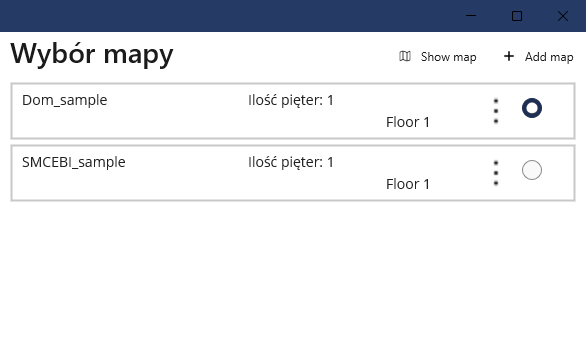
\includegraphics[scale=0.75]{MapPickerPage_light.png}}
    \caption{Ekran wyboru mapy w aplikacji "Navigator"}
    \label{img:MapPickerPage}
\end{figure}

\begin{figure}[ht]
    \centering
    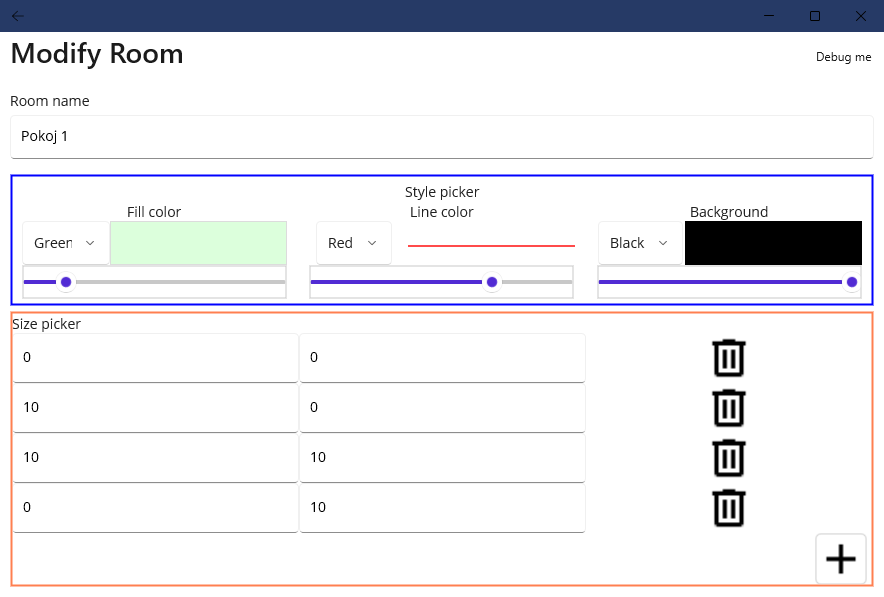
\includegraphics[width=\textwidth]{FeatureEditorPage_light.png}
    \caption{Ekran kreatora pokoju w aplikacji "Navigator"}
    \label{img:FeatureEditorPage}
\end{figure}


\begin{figure}[H]
    \centering
    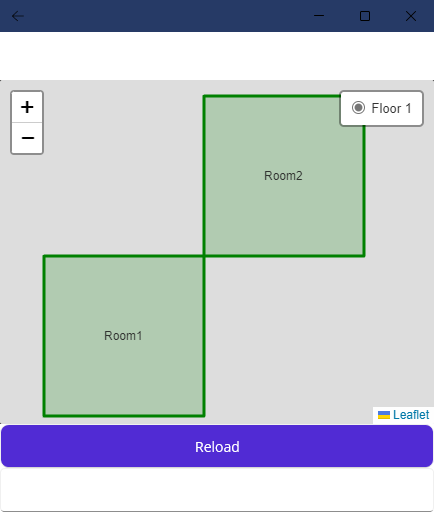
\includegraphics[width=0.55\textwidth]{MapDisplayPage_light.png}
    \caption{Ekran wyświetlający mapę w aplikacji "Navigator"}
    \label{img:MapDisplayPage}
\end{figure}
